\documentclass{../main.tex}{subfiles}
\begin{document}
\chapter{TCP:传输控制协议(初步)}
\section{引言}
% CRC和校验,只能检测有差错数据,但是无法纠正
% IP和UDP,没有实现纠正
% 以太网及其上的协议,提供一定次数尝试,失败则放弃
到目前为止,我们一直在讨论那些自身不包含可靠传递数据机制的协议。
它们可能回使用一种像校验或CRC这样的数学函数来检测接收到的有差错的数据,但是它们不尝试去纠正差错。
对于IP和UDP,根本没有实现差错纠正。
对于以太网和基于其上的其他协议,协议提供一定次数的尝试,如果还是不成功则放弃。

% 尽量避免信息在通信信道出错方法:
% 1. 差错纠正码
% 2. 重试,ARQ
通信媒介可能会丢失或改变被传递的信息,在这种环境下的通信问题已经被研究了多年。
关于这个课题的一些最重要的理论工作由克劳德\textperiodcentered 香农在1948年给出\cite{Shannon1948A}。
这些工作普及了术语``比特'',并成为\emph{信息理论}(information theory)领域的基础,
    帮助我们理解了在一个有损(可能会删除或改变比特)信道里可通过的信息量的根本限制,
信息理论与\emph{编码理论}(coding theory)的领域密切相关,编码理论提供不同的信息编码手段,从而使得信息能在通信信道里尽量免于出错。
使用\emph{差错校正码}(基本上是添加一些冗余的比特,使得即使某些比特被毁,真实的信息也可以被恢复过来)来纠正通信问题是处理差错的一种非常重要的方法。
另一种方法是简单地``尝试重新发送'',直到信息最终被接收。
这种方法,称为\emph{自由重复请求}(Automatic Repeat Request, ARQ),构成了许多通信协议的基础,包括TCP在内。


\subsection{ARQ和重传}
如果我们考虑的不只是单个通信信道,而是几个的多跳级联,我们会发现不只会碰到前面提到的那几种差错类型(分组比特差错),而且还会有更多其他的类型。
这些问题可能发生在中间路由器上,是几种在讨论IP时会遇到的问题:分组重新排序,分组复制,分组泯灭(丢失)。
在多跳通信信道(例如IP)上使用而设计的带纠错的协议必须要处理这些问题。
现在让我们探讨能处理这些问题的协议机制。在概括性地讨论这些之后,我们会探究它们是如何被TCP在互联网上使用的。

% 重发直到它被接收,关键点:
% 1. 怎样判定接收方已收到 ==> ACK
% 2. 和之前收到的是否相同 ==> 序列号
% 
% 引入ACK带来的问题:
% 1. 发送方对ACK应该等待多久
% 2. ACK丢失 ==> 重试(无法判定是ACK丢失还是分组丢失)
% 3. 接收到的分组数据有错 ==> 编码技术纠正或检测错误 ==> 收到错误的分组,不发送ACK
一个直接处理分组丢失(和比特差错)的方法是重发分组直到它被正确接收。这需要一种方法来判断: 
(1) 接收方是否已收到分组; (2) 接收方接收到的分组是否与之前发送方发送的一样。
接收方给发送方发信号以确定自己已经接收到一个分组,这种方法称为\emph{确认}(acknowledgment),或ACK。
最基本的形式是,发送方发送一个分组,然后等待一个ACK。当接收方接收到这个分组时,它发送对应的ACK。
当发送方接收到这个ACK,它再发送另一个分组,这个过程就这样继续。这里会有一些有意思的问题:
(1) 发送方对一个ACK应该对待多长时间? (2) 如果ACK丢失了怎么办? (3) 如果分组被接收到了,但是里面有错怎么办?

正如我们将看到的,第一个问题是挺深奥的。
决定去等待时间多长时间与发送方\emph{期待}(expect)为一个ACK等待多长时间有关。 % 没看懂,这是啥意思?
现在确定这个时间可能比较困难,因此我们推迟对这个技术的讨论,直到我们在后面(见第14章)详细讨论TCP。
第二个问题的答案比较容易: 如果第一个ACK丢失了,发送方不能轻易地把这种情况与原分组的情况区分开来,所以它简单地再次发送分组。
当然,这样的话,接收方可能会收到两个或更多的拷贝,因此必须准备好处理这种情况(见下一段)。
至于第三个问题,我们可以借助12.1节中提到的编码技术来解决。
使用编码技术来检测一个大的分组中的差错(有很大的概率)一般都很简单,仅使用比其自身小很多的一些比特即可纠正。
更简单的编码一般不能纠正差错,但是能检测它们。
这就是校验和CRC会如此受欢迎的原因。
然后,为了检测分组里的差错,我们使用一种校验和形式。
当一个接收方接收到一个含有差错的分组时,它不发送ACK。
最后,发送方重发完整到达的无差错的分组。

% 用序列号来去重
到目前为止即使这种简单的场景,接收方都可能接收到被传送分组的\emph{重复}(duplicate)副本。
这个问题要使用\emph{序列号}(sequence number)来处理。
基本上,在被源端发送时,每个唯一的分组都有一个新的序列号,这个序列号由分组自身一直携带着。
接收方可以使用这个序列号来判断它是否已经见过这个分组,如果见过则丢弃它。

% 停止和等待协议的吞吐性能低
到目前为止介绍的协议是可靠的,但是效率不太高。
如果从发送方到接收方传递即使一个很小的分组都要用很长时间(推迟或延迟)的话(如一秒或两秒,对卫星链路来说并非不正常),考虑一下那会怎样。
发送方可以注入一个分组到通信路径,然后停下来直到知道它收到ACK。
这个协议因此被称为``停止和等待''。
假设没有分组在传输中丢失和无可挽回地损害,该吞吐量性能(每单位时间发送在网络中的数据量)与$M/R$成正比,$M$是分组大小,$R$是往返时间(RTT)。
如果有分组丢失和损害的话,情况甚至更糟糕: “吞吐质”(每单位时间传送的有用数据量)明显比吞吐量要低。

% 等待导致性能差,允许多个分组进入网络以便于提升性能,多个分组会引入其他问题
对于不会损害和丢失太多分组的网络来说,低吞吐量的原因是网络经常没有处于繁忙状态。
情况与使用装配流水线时不出一个完整产品就不准新的工作进入类似,流水线大部分时间是空闲的。
我们进一步对比,很明显,如果我们允许同一时间有多个工作单元进入流水,就可以做的更好。
对网络通信来说也是一样的---如果我们允许多个分组同时进入网络,就可以使它``更繁忙'',从而得到更高的吞吐量。

% 带来的问题:
% 1. 发送方: 维持ACK的计时器、未确认分组的副本
% 2. 接收方: 区分分组是否收到、维护混乱顺序的分组
% 3. 发送方、接收方、网络基础设施性能不均衡问题
很明显,允许多个分组同时进入网络使事情变得复杂。
现在发送方必须不仅要决定什么时间注入一个分组到网络中,还要注入多少个。
并且必须要指出在等待ACK时,怎样维持计时器,同时还必须要保存每个还没确认的分组的一个副本以防需要重传。
接收方需要有一个更复杂的ACK机制:可以区分哪些分组已经收到,哪些还没有。
接收方可能需要一个更复杂的缓存(分组保存)机制---允许维护``次序杂乱''的分组
(那些比预想要先到的分组更早到达的分组,因为丢包和次序重排的原因),
除非简单地抛弃这些分组,而这样做是很没效率的。
还有其他一些没有这么明显的问题。
如果接收方的接收速率比发送方的发送速率要慢怎么办?
如果发送方简单地以很高的速率发送很多分组,接收方可能会因处理或内存的限制而丢掉这些分组。
中间的路由器也会有相同的问题。
如果网络基础设施处理不了发送方和接收方想要使用的数据发送率怎么办?


\subsection{分组窗口和滑动窗口}
为了解决所有这些问题,我们以假设每个分组有一个序列号开始,正如前面所描述的。
我们定义一个分组窗口(window)作为已被发送方注入但还未完成确认(如,发送方还从没收到它们的ACK)的分组(或者它们的序列号)的集合。
我们把这个窗口中的分组数量称为\emph{窗口大小}(window size)。
术语\emph{窗口}来自这样的想法:
如果你把在一个通信对话中发送的所有分组排成长长的一行,但只能通过一个小孔来观察它们,你就只能看到它们的一个子集---像通过一个窗口查看一样。
发送方的窗口(以及其他分组队列)可画图描述成图12-1那样。
\todo[inline]{图12-1 滑动窗口}

这个图显示了当前三个分组的窗口,整个窗口大小是3。
3号分组已经被发送和确认,所以由发送方保存的它的副本可以被释放。
分组7在发送方已经准备好,但还没被发送,因为它还没有``进入''窗口。
现在如果我们想象数据从发送方流到接收方,ACK开始以相反的方向流动,发送方可能下一步就接收到一个分组4的ACK。
当这发生时,窗口向右边``滑动''一个分组,意味着分组4的副本可以释放了,而分组7可以被发送了。
窗口的这种滑动给这种类型的协议增加了一个名字,\emph{滑动窗口}(sliding window)协议。

% 滑动窗口-发送方
% 结构: 1. 可被释放的分组 2. 等待ACK的分组 3. 未发送分组
% 滑动分组-接收方
% 结构: 1. 已被确认和接收的分组 2. 下一步期望的分组 3. 接收也因各种约束被丢弃的分组
这种滑动窗口方法可用于对付到目前为止描述过的许多问题。
一般来说,这个窗口结构在发送方和接收方都会有。
在发送方,它记录着哪些分组可被释放,哪些分组正在等待ACK,以及哪些分组还不能被发送。
在接收方,它记录着哪些分组已经被接收和确认,哪些分组是下一步期望的(和已经分配多少内存来保存它们),以及哪些分组即使被接收也将会因内存限制而被丢弃。
尽管窗口结构便于记录在发送方和接收方之间流动的数据,但是关于窗口应多大,
    或者如果接收方或者网络处理不过来发送方的数据率时会发生什么,它都没有提供指导建议。现在我们应该看看这些怎样关联在一起。


\subsection{变量窗口: 流量控制和拥塞控制}
为了处理当接收方相对发送方太慢时产生的问题,我们介绍一种方法,在接收方跟不上时会强迫发送方慢下来。
这称为\emph{流量控制}(flow control),该控制经常以下述两种方式之一来进行操作。
一种方式称\emph{基于速率}(rate-based)流量控制,它是给发送方指定某个速率,同时确保数据永远不能超过这个速率发送。
这种类型的流量控制最适合流应用程序,可被用于广播和组播发现(见第9章)。

另一种流量控制的主要形式叫\emph{基于窗口}(window-based)流量控制,是使用滑动窗口时最流行的方法。
在这种方法里,窗口大小不是固定的,而是允许随时间而变动的。
为了使用这种技术进行流量控制,必须有一种方法让接收方可以通知发送方使用多大的窗口。
这一般称为\emph{窗口通告}(window advertisement),或简单地称为\emph{窗口更新}(window update)。
发送方(即窗口通告的接收者)使用该值调整其窗口大小。
逻辑上讲,一个窗口更新是与我们前面讨论过的ACK分离的,但是实际上窗口更新和ACK是由同一个分组携带的,
    意味着发送方往往会在它的窗口滑动到右边的同时调整它的大小。

如果我们考虑到在发送方修改窗口大小会带来的影响,就可以很明显地知道这是怎样达到流量控制的。
在没收到它们中任何一个的ACK之前,发送方允许注入$W$个分组到网络中。
如果发送方和接收方足够快,网络中没有丢失一个分组以及有无穷的空间的话,
    这意味着通信速度率正比于$(SW/R)$ b/s,这里$W$是窗口大小,$S$是分组大小(按比特算),$R$是往返时间(RTT)。
当来自接收方的窗口通告夹带着发送方的值$W$时,那么发送方的全部速率就被限制而不能超越接收方。
这种方法可以很好地保护接收方,但是对于中间的网络呢?
在发送方和接收方之间可能会有有限内存的路由器,它们与低速网络链路抗争着。
当这种情况出现时,发送方的速率可能超过某个路由器的能力,从而导致丢包。
这由一种特殊的称为\emph{拥塞控制}(congestion control)的流量控制形式来处理。

拥塞控制设计发送方减低速度以至于压垮其与接收方之间的网络。
回想我们关于流量控制的讨论,我们使用一个窗口通告来告之发送方于接收方减慢速度。
这称为\emph{明确}(explicit)发信,因为有一个协议字段专用于通知发送方正在发生什么。
另一个选项可能被发送方用于\emph{猜测}(guess)它需要慢下来。
这种方法涉及\emph{隐性}(implicit)发信---涉及根据其他某些证据来决定减慢速度。

数据报类型的网络或更一般的与之关联的排队理论(queuing theory)中的拥塞控制问题仍然是这些年的一个主要研究课题,它甚至不太可能完全解决所有情况。
在这里讨论关于流量控制的所有选择和方法也不现实。
有兴趣的读者可参考\cite{Jain1990Congestion}、\cite{1997An}和\cite{Kleinrock1975Queueing}。
在第16章我们将更详细地探讨实际用于TCP中的拥塞控制技术,以及这些年来出现的许多变体。


\subsection{设置重传时间}
基于重传的可靠协议的设计者要面对一个最重要的性能问题是,要等待多久才能判定一个分组已丢失并将它重发。
用另一种方式说,重传超时应该是多大?
直观上看,发送方在重发一个分组之前应等待的时间量大概是下面时间的总和:
发送分组所用的时间、接收方处理它和发送一个ACK所用的时间、ACK返回到发送方所用的时间以及发送方处理ACK所用的时间。
不幸的是,实际上这些时间没有一个是可以确切知道的。
更糟的是,它们中的某些或全部会随着来自终端主机或路由器的额外负载的增加或减少而随时改变。

让用户去告诉协议实现在所有情况下的每个时刻应取什么超时时间(或使它们保持最新),这是不现实的,一个更好的策略是让协议实现尝试去估计它们。
这称为\emph{往返时间估计}(round-trip-time estimation),这是一个统计过程。
总的来说,选择一组RTT样本的样本均值作为真实的RTT是最有可能的。
注意到这个平均值很自然地会随着时间而改变(它不是静态的),因为通信穿过网络的路径可能会改变。

作出对RTT的一些估计之后,关于设置实际的用于触发重传的超时取值问题依然存在。
如果我们回想一下均值的定义,会知道它绝不可能是一组样本的均值(除非它们全部一样)。
所以,把重传计时器的值设置成正好等于平均估计量是不合理的,因为很有可能许多实际的RTT将会比较大,从而会导致不必要的重传。
很明显,超时应该设置成比均值要大的某个值,但是这个值与均值的确切关系是什么(或者甚至直接就使用均值)还不清楚。
超时设置得太大也是不可取的,因为这反过来会导致网络变得空闲,从而降低吞吐量。
对于这个话题的进一步探究留到第14章,我们在那里会探讨TCP是怎样实际地处理这个问题的。


\section{TCP的引入}
我们现在对影响可靠传输的问题有了大体的了解,下面看一下它们是怎样在TCP中体现的,以及TCP会给互联网应用程序提供什么类型的服务。
我们还要查看TCP头部中的字段,了解有多少个到目前为止我们已经见过的概念(如ACK、窗口通告)可在头部描述中捕捉到。
在随后的章节,我们会更详细地检查所有这些头部字段。

我们对TCP的描述从这一章开始,并在接下来的五章中继续讨论。
第13章描述一个TCP连接是怎样建立和结束的。
第14章详细说明TCP是怎样估计每个链接的RTT和怎样基于这个估计设置重传超时的。
第15章考察正常的数据传输,以``交互式''应用程序开始(例如聊天程序),然后是窗口管理和流量控制,
    这被应用于交互式和``大块''数据流(比如文件传输)两种应用程序以及TCP的\emph{紧急机制}(urgent machanism)---
    它允许发送方指定数据流中的某些数据作为特殊数据。
第16章考察了TCP里的拥塞控制算法,这些算法在网络很繁忙中的时候帮助降低丢包率。
这一章还讨论了一些改动,这些改动被提出来以增加快速网络的吞吐量和改进易损耗(如无线)网络的弹性。
最后,第17章显示TCP如何在没有数据流动时保持连接的活动性。
\todo[inline]{相关参考}


\subsection{TCP服务模型}
虽然TCP和UDP使用相同的网络层(IPv4或IPv6),但是TCP给应用程序提供了一种与UDP完全不同的服务。
TCP提供了一种\emph{面向连接的}(connection-oriented)、可靠的字节流服务。
术语``面向连接的''是指使用TCP的两个应用程序必须在它们交换数据之前,通过相互联系来建立一个TCP连接。
最典型的比喻就是拨打一个电话号吗,等待另一方接听电话并说``喂'',然后再说``找谁?''。
这正是一个TCP连接的两个端点在互相通信。像广播和组播(见第9章)这些概念在TCP中都不存在。

TCP提供一种字节流抽象概念给应用程序使用。
这种设计方案的结果是,没有由TCP自动插入的记录标志和消息边界(见第1章)。
一个记录标志对应着一个应用程序的写范围指示。
如果应用程序在一端写入10字节,随后写入20字节,再随后写入50字节,那么在连接的另一端的应用程序是不知道每次写入的字节是多少的。
例如,另一端可能会以每次20字节分四次读入这80字节或以其他一些方式读入。
一端给TCP输入字节流,同样的字节流会出现在另一端。
每个端点独立选择自己的读和写大小。

TCP根本不会解读字节流里的字节内容。
它不知道正在交换的数据字节是不是二进制数据、ASCII字符、EBCDIC字符或其他东西。
对这个字节流的解读取决于连接中的每个端点的应用程序。
尽管不再推荐使用,可TCP确实是支持以前提到过的紧急机制。


\subsection{TCP中的可靠性}
通过使用刚才描述的那些技术的特定变种,TCP提供了可靠性。
因为它提供了一个字节流接口,TCP必须把一个发送应用程序的字节流转换成一组IP可以携带的分组。
这被称为\emph{组包}(packetization)。
这些分组包含序列号,
    该序列号在TCP中实际代表了每个分组的第一个字节在整个数据流中的字节偏移,而不是分组号。
这允许分组在传送中是可变大小的,并允许它们组合,称为\emph{重新组包}(repacketization).
应用程序数据被打散成TCP认为的最佳大小的块来发送,
    一般使得每个报文段按照不会被分片的单个IP层数据包的大小来划分。
这与UDP不同,应用程序每次写入通常就产生一个UDP数据,其大小就是写入的那么大(加上头部)。
由TCP传给IP的块称为\emph{报文段}(segment, 见图12-2)。
在第15章我们会看到TCP如何判定一个报文段的大小。

TCP维持了一个强制的校验和,该校验和涉及它的头部、任何相关应用程序数据和IP头部的所有字段。
这是一个端到端的伪头部,它用于检测传送中引入的比特差错。
如果一个带无效校验和的报文段到达,那么TCP会丢弃它,不为被丢弃的分组发送任何确认。
然而,TCP接收端可能会对一个以前的(已经确认的)报文段进行确认,以帮助发送方计算它的拥塞控制(第16章)。
TCP校验和使用的数学函数与其他互联网协议(UDP、ICMP等)一样。
对于大数据的传送,对这个校验和是否不够强壮的担心是存在的,
    所以仔细的应用程序应该应用自己的差错保护方法(如,更强的校验和或CRC),
    或者使用一种中间层来达到同样的效果。

当TCP发送一组报文段时,它通常设置一个重传计时器,等待对方的确认接收。
TCP不会为每个报文段设置一个不同的重传计时器。
相反,发送一个窗口的数据,它只设置一个计时器,当ACK到达时再更新超时。
如果有一个确认没有及时接收到,这个报文段就会被重传。
在第14章我们将更详细地查看TCP的自适应超时和重传策略。

当TCP接收到连接的另一端的数据时,它会发送一个确认。
这个确认可能不会立即发送,而一般会延迟片刻。
TCP使用的ACK是\emph{累积}的,从某种意义上来讲,
    一个指示字节号$N$的ACK暗示着所有直到$N$的字节(但不包括$N$)已经成功被接收了。
这对于ACK丢失来说带来了一定的鲁棒性---如果一个ACK丢失,很有可能后续的ACK就足以确认前面的报文段了。

TCP给应用程序提供一种\emph{双工}服务。
这就是说数据可向两个方向流动,两个方向互相独立。
因此,连接的每个端点必须对每个方向维护数据流的一个序列号。
一旦建立了一个连接,这个连接的一个方向上的包含数据流的每个TCP报文段也包含了相反方向上的报文段的一个ACK。
每个报文段也包含了一个窗口通告以实现相反方向上的流量控制。
为此,在一个连接中,当一个TCP报文段到达时,窗口可能向前滑动,窗口大小可能改变,同时新数据可能已到达。
正如我们将在第13章所见,一个完整的TCP连接是双向和对称的,数据可以在两个方向上平等地流动。

使用序列号,一个TCP接收端可丢弃重复的报文段和记录以杂乱次序到达的报文段。
回想一下,任何反常情况都会发生,因为TCP使用IP来传递它的报文段,IP不提供重复消除或保证次序正确的功能。
然而,因为TCP是一个字节流协议,TCP绝不会以杂乱的次序接收\emph{应用程序}发送数据。
因此,TCP接收端可能会被迫先保持大序列号的数据不交给应用程序,直到缺失的小序列号的报文段(一个``洞'')被填满。

我们现在开始观察TCP的一些细节。
这一章只介绍TCP的封装和头部结构,其他细节出现在后面的五章中。
TCP可以与IPv4或IPv6使用,同时它使用的伪头部(与UDP的类似)在IPv4中和IPv6中都是强制使用的。


\section{TCP头部和封装}
图12-2显示了TCP在IP数据报中的封装。
\todo[inline]{图12-2 TCP在IP数据报中的封装}

头部本身明显要比在第10章我们见过的UDP的头部更复杂。
这并不很令人惊讶,因为TCP是一个明显更复杂的协议,它必须保持连接的每一端知道(同步)最新状态。
如图12-3所示。
\todo[inline]{图12-3 TCP头}

每一个TCP头部包含了源和目的端口号,这两个值与IP头部中的源和目的IP地址一起,唯一地标识了每个连接。
在TCP术语中,一个IP地址和一个端口的组合有时候被称为一个\emph{端点(endpoint)}或\emph{套接字(socket)}。
后者出现在\cite{1981Transmission}中,最终被Berkeley系列的网络通信编程接口所采用(现在经常被称为``Berkeley套接字'')。
每个TCP连接由一对套接字或端点(四元组,由客户机IP地址、客户机端口号、服务器IP地址以及服务器端口号组成)唯一地标识。
这个事实在我们观察一个TCP服务器是如何做到与多个客户机通信的时候将会变得非常重要(见第13章)。

\emph{序列号(Sequence Number)}字段标识了TCP发送端到TCP接收端的数据流的一个字节,
    该字节代表着包含该序列号的报文段的数据中的第一个字节。
如果我们考虑在两个应用程序之间的一个方向上流动的数据流,TCP给每个字节赋予一个序列号
这个序列号是一个32位的无符号数,到达$2^{32}-1$后再循环回到0。
因为每个被交换的字节都已被编号,\emph{确认号}字段(也简称ACK号或ACK字段)包含的值是该确认号的发送方期待接收的下一个序列号。
即最后被成功接收的数据字节的序列号加1。
这个字段只有在ACK位字段被启用的情况下才有效,这个ACK位字段通常用于除了初始和末尾报文段之外的所有报文段。
发送一个ACK和发送任何一个TCP报文段的开销是一样的,因为那个32位的ACK号字段一直都是头部的一部分,ACK位字段也一样。

当建立一个新连接时,从客户机器发送至服务器的第一个报文段的SYN位字段被启用。
这样的报文段被称为\emph{SYN报文段},或简单地称为SYN。
然后\emph{序列号}字段包含了在本次连接的这个方向上要使用的第一个序列号,后续序列号和返回的ACK号也在这个方向上(回想一下,连接是双向的)。
注意这个数字\emph{不是0和1},而是另外一个数字,经常是随机选择的,称为\emph{初始序列号(Initial Sequence Number, ISN)}。
ISN不是0和1,是因为这是一种安全措施,将会在第13章讨论。
发送在本次连接的这个方向上的数据的第一个字节的序列号是ISN加1,因为SYN位字段会\emph{消耗}一个序列号。
正如我们稍后将见到的,消耗一个序列号也意味着使用重传进行可靠传输。
因此,SYN和应用程序字节(还有FIN,稍后我们将见到)是被可靠传输的。
不消耗序列号的ACK则不是。

TCP可以被描述为``一种带累积正向确认的滑动窗口协议''。
\emph{ACK号}字段被构建用于指明在接收方已经顺序收到的最大字节(加1)。
例如,如果字节1~1024已经接收成功,而下一个报文段包含字节2049~3072,
    那么接收方不能使用规则的ACK号字段去发信告诉发送方它接收到了这个新报文段。
然而,现代TCP有一个\emph{选择确认(Selective ACKnowledgment, SACK)}选项,可以允许接收方告诉发送方它正确地接收到了次序杂乱的数据。
当于一个具有\emph{选择重发(selective repeat)}能力的TCP发送方搭配时,就可以实现性能的显著改善。
在第14章我们将会看到TCP是如何使用\emph{重复确认(duplicate acknowledgments)}以帮助它的拥塞控制和差错控制过程的。

\emph{头部长度}字段给出了头部的长度,以32位字为单位。
它是必须的,因为\emph{选项}字段的长度是可变的。
作为一个4位的字段,TCP被限制为只能带60字节的头部。
而不带选项,大小是20字节。

当前,为TCP头部定义了8位的字段可,尽管一些老的实现只理解它们中的最后6位。
它们中的一个或多个可被同时启用。
我们在这里大致提一下它们的用法,在后面几章里再对每个进行详细的讨论。
\begin{enumerate}
    \item CWR --- 拥塞窗口减(发送方降低它的发送速率);见第16章。
    \item ECE --- ECN回显(发送方接收到了一个更早的拥塞通告);见第16章。
    \item URG --- 紧急(紧急指针字段有效---很少被使用);见第15章。
    \item ACK --- 确认(确认号字段有效---连接建立以后一般都是启用状态);见第13章和第15章。
    \item PSH --- 推送(接收方应尽快给应用程序传送这个数据---没被可靠地实现或用到);见第15章。
    \item RST --- 重置连接(连接取消,经常是因为错误);见第13章。
    \item SYN --- 用于初始化一个连接的同步序列号;见第13章。
    \item FIN --- 该报文段的发送方已经结束向对方发送数据;见第13章。
\end{enumerate}

TCP的流量控制由每个端点使用\emph{窗口大小}字段通告一个窗口大小来完成。
这个窗口大小是字节数,从ACK号指定的,也是接收方想要接收的那个字节开始。
这是一个16位的字段,限制了窗口大小到65535字节,从而限制了TCP的吞吐量性能。
在第15章我们将看到窗口缩放(Window Scale)选项可允许对这个值进行缩放,给高速和大延迟网络提供了更大的窗口和改进性能。

TCP\emph{校验和}字段覆盖了TCP的头部和数据以及头部中的一些字段,
    使用一个与我们在第8章和第10章讨论的ICMPv6与UDP使用的相类似伪头部进行计算。
这个字段是强制的,由发送方进行计算和保存,然后由接收方验证。
TCP校验和的计算算法与IP、ICMP和UDP(``互联网'')校验和一样。

\emph{紧急指针(Urgent Pointer)}字段只有在URG位字段被设置时才有用。
这个``指针''是一个必须要加到报文段的\emph{序列号}字段上的正偏移,以产生紧急数据的\emph{最后}一个字节的序列号。
TCP的紧急机制是一种让发送方给另一端提供特殊标志数据的方法。

最常见的\emph{选项}字段就是``最大段大小''选项,称为MSS。
连接的每个端点一般在它发送的第一个报文段(为了建立该连接,SYN位字段被设置的那个报文段)上指定这个选项。
MSS指定该选项的发送着在相反方向上希望接收到的最大报文段的最大值。
在第13章我们将更详细地描述MSS选项,并在第14章和第15章描述其他一些TCP选项。
我们考察的其他普通选项还包括SACK、时间戳和窗口缩放。

在图12-2中我们主要到TCP报文段的数据部分是可选的。
在第13章我们将看到的一个连接被建立和终止时,交换的报文段只包含了TCP头部(带或不带选项)而没有数据。
如果这个方向上没有数据被传输,那么一个不带任何数据的头部也会被用于确认接收到的数据(称为一个\emph{纯(pure)}ACK),
    同时通知通信方改变窗口大小(称为一个\emph{窗口更新(window update)})。
当一个报文段可不带数据发送时,超时操作会因此而产生一些新情况。


\section{总结}
在有损通信信道上提供可靠通信的问题已经被研究了许多年。
处理差错的两种主要方法是差错矫正码和数据重传。
使用重传的协议必须也要处理数据丢失,经常通过设置一个计时器来进行,同时还必须要给接收方安排一些方法来告知发送方它已接收了什么。
判定等待一个ACK要多长时间是比较棘手的,因为合适的时间会随着网络路由或端点上负载的变动而改变。
现代协议用基于这些测量值的一些函数来估计往返时间以及设置重传计时器。

不考虑设置重传计时器的话,当同一时间只有一个分组在网络中时,重传协议时很简单的,
    但对于延迟很高的网络,它们的性能很差。
为了更有效率,在一个ACK被接收到之前,多个分组必须被注入网络中。
这种方法更有效率,但也更复杂。
一种管理这些复杂性的典型方法时使用滑动窗口,其中分组用序列号标志,窗口大小限制分组数量。
当窗口大小基于来自接收方或其他信号(比如被丢弃的分组)的回馈而改变时,流量控制和拥塞控制两者就都被实现了。

TCP提供一种可靠,面向连接、字节流、传输层的服务(通过使用许多这些技术而构建)。
我们简单地看了TCP头部里的所有字段,了解到它们中的大多数都与这些可靠传递的抽象概念有着直接关系。
我们将在接下来的章节里详细考察它们。
TCP把应用程序数据组包成报文段,发送数据时设置超时,确认被其他端点接收到的数据,给次序杂乱的数据进行重新排序,
    丢弃重复的数据,提供端到端的校验和。
TCP在互联网中被广泛应用,不仅许多流行的应用程序使用它,
    例如HTTP、SSH/TLS、NetBIOS(NBT---NetBIOS over TCP)、Telnet、FTP以及电子邮件(SMTP),
    许多分布式文件共享程序(如,BitTorrent,Shareaza)也使用它。

% \begin{compactenum}[1.]
%     \item 接收方是否已收到分组;
%     \item 接收方接收到的分组是否与之前发送方发送的一样。
% \end{compactenum}

\chapter{TCP连接管理}
\section{引言}
TCP是一种\emph{面向连接}的单播协议。
在发送数据之前,通信双方必须在彼此间建立一条连接。
本章将详细地介绍TCP连接的概念,以及它的建立与终止过程。
如前文所述,TCP服务模型是一个字节流。
TCP必须检测并修补所有在IP层(或下面的层)产生的数据传输问题,比如丢包、重复以及错误。

由于需要对连接状态进行管理(通信双方都需要维护连接的信息),TCP被认为是一个比UDP(第10章)复杂的多的协议。
UDP是一种无连接的协议,因此它不需要连接的建立和终止过程。
与UDP相比,TCP在妥善处理多种TCP状态时需要面对大量的细节问题,
    比如一个连接何时建立、正常地终止、以及在无警告的情况下重新启动。
因此,这也被认为是两个协议的主要区别之一。
在后续章节,我们将探讨一旦建立连接并传输数据将会发生什么。

在连接的过程中中。通信双方需要交换一些选项。
这些选项被认为是连接的参数。
一些选项只被允许在连接建立时发送,而其他一些选项则能够稍后发送。
根据第12章的介绍,TCP头部已设置了一个有限的空间(40字节)来处理这些选项。


\section{TCP连接的建立与终止}
一个TCP连接由一个4元组构成,它们分别是两个IP地址和两个端口号。
更准确地说,一个TCP连接是由一对端点或套接字构成,其中通信的每一端都由一对(IP地址、端口号)所唯一标识。

一个TCP连接通常分为3个阶段: 启动、数据传输(也称为``连接已建立'')和推出(关闭)。
下文我们将会发现正确地处理上述三个阶段之间的转换是创建一个强健的TCP连接的困难所在。
图\ref{fig:create-destroy-connection}显示了一个典型的TCP连接的建立和关闭过程(不包括任何数据传输)。

图\ref{fig:create-destroy-connection}中的时间轴描绘了一个连接建立改成的相关事宜。为了建立一个TCP连接,需要完成以下步骤:
\begin{enumerate}
    \item 主动开启者(通常称为客户端)发送一个SYN报文段(即一个在TCP头部的SYN位字段置位的TCP/IP数据包),
        并指明自己想要连接的端口号和它的客户端初始序列号(记为ISN(c),参见13.2.3节)。
        通常,客户端还会借此发送一个或多个选项(参见13.3节)。客户端需发送的这个SYN报文段称作段1。
    \item 服务器也发送自己的SYN报文段作为响应,并包含了它的初始序列号(记为ISN(s))。该段称作段2。
        此外,为了确认客户端的SYN,服务器将其包含的ISN(c)数值+1后作为返回的ACK数值。
        因此,每发送一个SYN,序列号就会自动加1。这样如果出现丢失的情况,该SYN段将会重传。
    \item 为了确认服务器的SYN,客户端将ISN(s)的数值+1后作为返回的ACK数值。这称作段3。    
\end{enumerate}
\begin{center}
    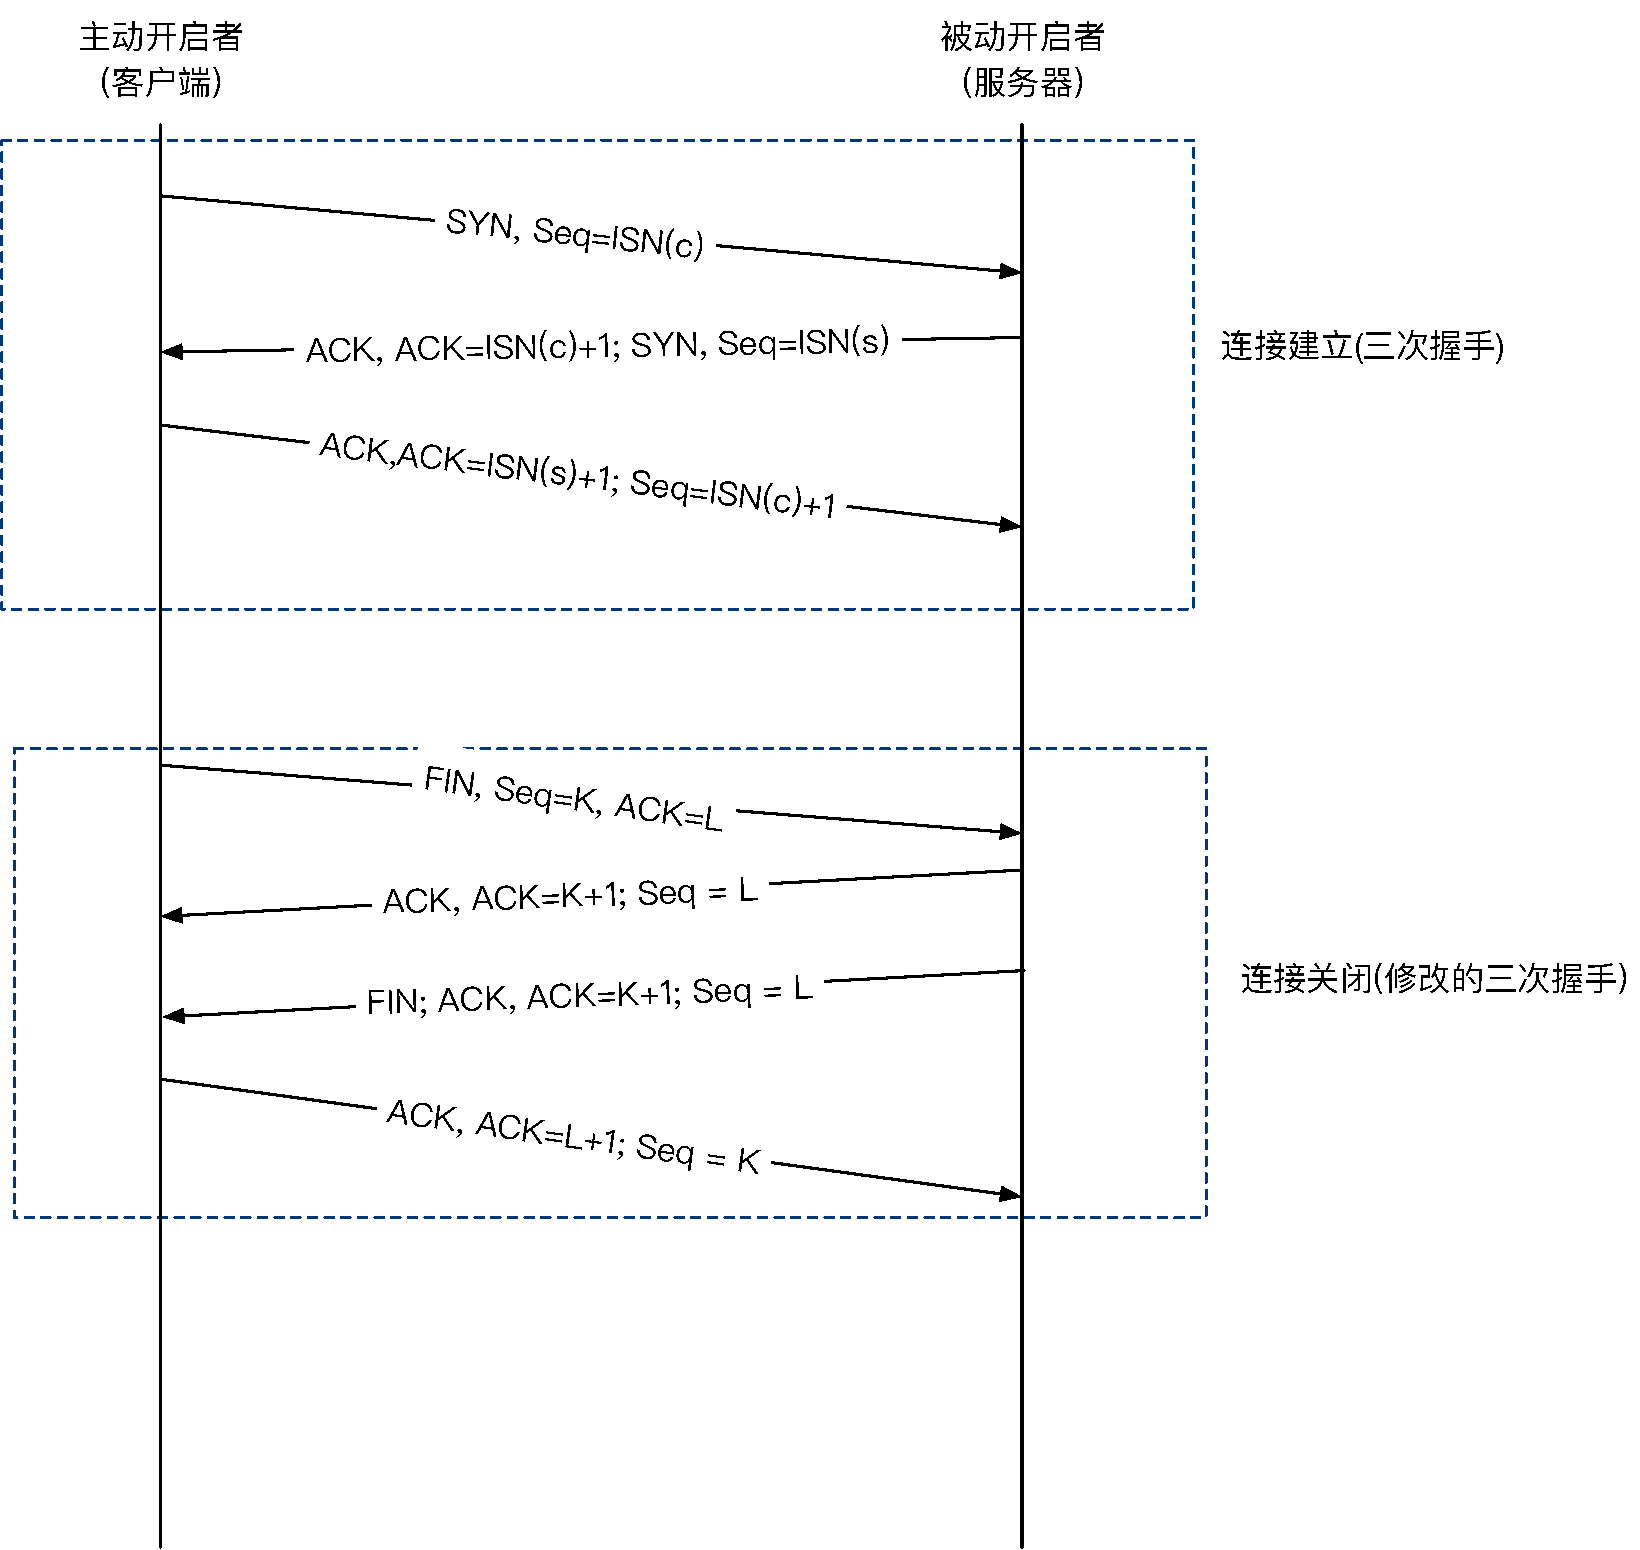
\includegraphics[width=0.8\textwidth]{res/cs/net/images/create-destroy-connection.pdf}
    \captionof{figure}{
        一个普通TCP连接的建立与终止
    }
    \label{fig:create-destroy-connection}
\end{center}

如图\ref{fig:create-destroy-connection}所示,在一个普通的TCP连接建立与终止中。
通常由客户端负责发起一个三次握手过程。
在该过程中,客户端与服务器利用SYN报文段交换彼此的初始序列号(包括客户端的初始序列号和服务器的初始序列号)。
在通信双方都发送了一个FIN数据包并收到来自对方的相应的确认数据包后,该连接终止。

通过发送上述3个报文段就能够完成一个TCP连接的建立。
它们也常称作\emph{三次握手}。
三次握手的目的不仅在于让通信双方了解一个连接正在建立,还在于利用数据包的选项来承载特殊的信息,
    交换\emph{初始序列号(Initial Sequence Number, ISN)}。

发送首个SYN的一方被认为是主动地打开一个连接。
如上文所述,它通常是一个客户端。
连接的另一方会接收这个SYN,并发送下一个SYN,因此它是被动地打开一个连接。
通常,这一方称为服务器。
(13.2.2节将会介绍一种客户端与服务端同时打开一个连接的情况。这种情况可以作为上文所介绍内容的补充,但非常少见。)

\begin{tcolorbox}[title={注意}]
    TCP的SYN段也能够承载应用数据。
    由于伯克利套接字API不支持这种方式,因此它也很少为人所用。
\end{tcolorbox}

图\ref{fig:create-destroy-connection}还描绘了一个TCP连接是怎样关闭的(也称为清除或终止)。
连接的任何一方都能够发起一个关闭操作。
此外,该过程还支持双方同时关闭连接的操作,但这种情况非常少见。
在传统的情况下,负责发起关闭连接的通常是客户端(如图\ref{fig:create-destroy-connection}所示)。
然而,一些服务器(例如Web服务器)在对请求作出响应之后也会发起一个关闭操作。
通常一个关闭操作是由应用程序提出关闭连接的请求而引发的(例如使用系统调用close())。
TCP协议规定通过发送一个FIN段(即FIN位字段置位的TCP报文段)来发起关闭操作。
只有当连接双方都完成关闭操作后,才构成一个完整关闭:

1. 连接的主动关闭者发送一个FIN段指明接收者希望看到的自己的当前序列号($K$, 如图\ref{fig:create-destroy-connection}所示)。
FIN段还包含了一个ACK用于确认对方最近一次发来的数据(图\ref{fig:create-destroy-connection}中标记为L)。

2. 连接的\emph{被动关闭者}将$K$的数值加一作为响应的ACK值,
    以表明它已经成功接收到主动关闭者发送的FIN。
此时,上层的应用程序会被告知连接另一端已经提出了关闭的请求。
通常,这将导致应用程序发起自己的关闭操作。
接着,被动关闭者将身份转换为主动关闭者,并发送自己的FIN。该报文段的序列号为$L$。

3. 为了完成连接的关闭,最后发送的报文段还包含一个ACK用于确认上一个FIN。
值得注意的是,如果出现FIN丢失的情况,那么发送方将重新传输直到接收到一个ACK确认为止。

综上所述,建立一个TCP连接需要3个报文段,而关闭一个TCP连接需要4个报文段。
TCP协议还支持连接处于半开启状态(参见13.6.3节),但这种情况并不常见。
存在上述半开启状态的原因在于TCP的通信模型是双向的。
这也意味着在两个方向中可能会出现只有一个方向正在进行数据传输的情况。
TCP\emph{半关闭}操作是指仅关闭数据流的一个传输方向,而两个半关闭操作合在一起就能够关闭整个连接。
因此TCP协议规定通信的任何一方在完成数据发送任务后就能够发送一个FIN。
当通信的另一方接收到这个FIN时,就会告知应用程序对方已经终止了对应方向的数据传输。
由此可见,当程序发布关闭操作请求后,通信双方往往通过发送FIN段来关闭双向的数据传输。

如上文所述,7个报文段时每一个TCP连接在正常建立与关闭时的基本开销(下文还会介绍一些突然关闭TCP连接的方式)。
因此当只需要交换少量的数据时,一些应用程序更愿意选择在发送与接收数据之前不需要建立连接的UDP协议。
然而,这些应用程序也会面对由此引入的错误修复、拥塞管理以及流量控制等诸多问题。


\subsubsection{TCP半关闭}
如前文所述,TCP支持半关闭操作。
虽然一些应用需要此项功能,但它并不常见。
为了实现这一特性,API必须为应用程序提供一种基本的表达方式。
例如,应用程序表明``我已经完成了数据的发送工作,并发送一个FIN给对方,
    但是我仍然希望接收来自对方的数据直到它发送一个FIN给我''。
伯克利套接字的API提供了半关闭操作。
应用程序只需要调用shutdown()函数来代替基本的close()函数,就能实现上述操作。
然而,绝大部分应用程序仍然会调用close()函数来同时关闭一条连接的两个传输方向。
图13-2展示了一个正在使用的半关闭示例。
图中左侧的客户端负责发起半关闭操作,然而在实际应用中,通信的任何一方都能完成这项工作。

首先发送的两个报文段与TCP正常关闭完全相同:
初始者发送的FIN,接着是接收者回应该FIN的ACK。
由于接收到半关闭的一方仍能发送数据,因此图13-2中的后续操作与图\ref{fig:create-destroy-connection}不同。
虽然图13-2在ACK之后只描述了一个数据段的过程,
    但实际应用时可以传输任意数量的数据段(第15章将会详细地讨论数据段的交换与确认细节)
当接收半关闭的一方完成数据发送后,它将会发送一个FIN来关闭本方的连接,同时向发起半关闭的应用程序发出一个文件尾指示。
当第2个FIN被确认之后,整个连接完全关闭。 


\subsubsection{同时打开与关闭}
虽然两个应用程序同时主动打开连接看似不太可能,但是在特定安排的情况下是有可能实现的。
通信双方在接收到来自对方的SYN之前必须先发送一个SYN;
两个SYN必须通过网络送达对方。
该场景还要求通信双方都拥有一个IP地址与端口号,并且将其告知对方。
上述情况十分少见(第7章介绍的防火墙``打洞''技术除外),一旦发生,可称其为\emph{同时打开}。

例如,主机A的一个应用程序通过本地的7777端口向主机B的8888端口发送一个主动打开请求,
    与此同时主机B的一个应用程序也通过本地8888端口向主机A的7777端口提出一个主动打开请求,
    此时就会发生一个同时打开的情况。
这种情况不同于主机A的一个客户端连接主机B的一个服务器,
    而同时又有主机B的一个客户端连接主机A的一个服务器的情况。
在这种情况下,服务器始终是连接的被动打开者而非主动打开者,而各自的客户端也会选择不同的端口号打开。
因此,它们可以被区分为两个不同的TCP连接。
图13-3显示了在一个同时打开过程中报文段的交换情况。

一个同时打开过程需要交换4个报文段,比普通的三次握手增加了一个。
由于通信双方都扮演了客户端和服务器的角色,因此不能将任何一方称作客户端与服务器。
同时关闭并没有太大区别。
如前文所述,通信一方(通常是客户端,但不一定总是)提出主动关闭请求,并发送首个FIN。
在同时关闭中,通信双方都会完成上述工作。
图13-4显示了在一个同时关闭中需要交换的报文段。

同时关闭需要交换与正常关闭相同数量的报文段。两者真正的区别在于报文段序列是交叉的还是顺序的。
下文将会介绍TCP实现中同时打开与同时关闭操作使用特殊状态这一不常见的方法。


\subsubsection{初始序列号}
当一个连接打开时,任何拥有何时的IP地址、端口号、符合逻辑的序列号(即在窗口中)
    以及正确校验和的报文段都会被对方接收。
然而,这也引入了另外一个问题。
在一个连接中,TCP报文段在经过网络路由器后可能会存在延迟抵达与排序混乱的情况。
为了解决这一问题,需要仔细选择初始序列号。本届将详细介绍这一过程。

在发送用于建立连接的SYN之前,通信双方会选择一个初始序列号。
初始序列号随着时间改变而改变,因此每一个连接都拥有不同的初始序列号。
RFC0793指出初始序列号可被视为一个32位的计数器。
该计数器每4微妙加1。
此举的目的在于为一个连接的报文段安排序列号,以防止出现与其他连接的序列号重叠的情况。
尤其是对于同一连接的两个不同的实例而言,心的序列号也不能出现重叠的情况。

由于一个TCP连接是被一对端点所唯一标识的,其中包括由2个IP地址与2个端口构成的4元组,
    因此即便是同一个连接也会出现不同的实例。
如果连接由于某个报文段的长时间延迟而被关闭,然后又以相同的4元组被重新打开,
    那么可以相信延迟的报文段有会被视为有效数据而重新进入新连接的数据流中。
上述情况十分会令人十分烦恼。
通过采取一些步骤来避免连接实例间的序列号重叠问题,能否将风险降到最低。
即便如此,
    一个对数据完整性有较高要求的应用程序
    也可以在应用层利用CRC或校验和保证所需数据在传输过程中没有出现任何错误。
在任何情况下这都是一种很好的方法,并已普遍用于大文件传输。

如前文所述,一个TCP报文段只有同时具备连接的4元组与当前活动窗口的序列号,
    才会在通信过程中被对方认为是正确的。
然而,这也从另一个侧面反映了TCP的脆弱性:
如果选择合适的序列号、IP地址以及端口号,
    那么任何人都能伪造一个TCP报文段,从而打断TCP的正常连接。
一种抵御上述行为的方法是使初始化序列号(或者临时窗口号)变得相对难以猜出,
    而另一种方法则是加密(参见第18章)。

% Linux: 时钟 + 随机偏移量(散列函数生成,散列函数5min改变一次)
现代系统通常采用半随机的方法选择初始序列号。
证书报告CA-2001-09讨论了这一方法的具体实现细节。
Linux系统采用一个相对复杂的过程来选择它的初始序列号。
它采用了基于时钟的方案,并且针对每一个连接为时钟设置随机的偏移量。
随机偏移量是在连接标识(即4元组)的基础上利用加密散列函数得到的。
散列函数的输入每隔5分钟就会改变一次。
在32位初始序列号中,最高的8位是一个保密的序列号,而剩余的各位则由散列函数生成。
上述方法所生成的序列号很难被猜出,但依然会随着时间而逐步增加。
据报告显示,Windows系统使用了一种基于RC4的类似方案。


\subsubsection{例子}
前文介绍了一个TCP连接的建立和退出过程,本节将从数据包(分组)的角度进一步介绍相关细节。
为此我们尝试对邻近的Web服务器进行TCP连接。
该主机的IPv4地址为10.0.0.2,而客户端采用了基于Windows的Telnet应用。

telnet命令是建立在TCP连接的基础上的。
在上述例子中,该TCP连接必须与服务器的IPv4地址10.0.0.2以及http或Web服务的端口号(80端口)相关联。
当Telent应用程序连接23以外的端口(Telnet协议的众所周知端口以外的端口),它将不能用于应用协议。
它仅仅将自己的字节输入拷贝至TCP连接中,反之亦然。
当一个Web服务器接收到进入的连接请求时,它首先需要等待对Web页面的请求。
在这种情况下,我们不能提供这样的请求,因此服务器不会产生任何数据。
这些均符合我们的期望,因为我们只对连接建立与终止过程中的数据包交换感兴趣。
图13-5展示了Wireshark软件对该命令所产生的报文段的输出结果。

如图13-5所示,客户端发送的SYN报文段所包含的初始序列号为685506836,广告窗口为65535。
该报文段还包含了若干其他选项。
13.3节将详细地讨论这些选项。
第二个报文段既包含了服务器的SYN还包含了对客户端请求的ACK确认。
它的序列号(服务器的初始序列号)为1479690171,ACK为685506837。
ACK号仅比客户端的初始序列号大1,说明服务器已经成功接收到了客户端的初始序列号。
该报文段同样也包含了一个广告窗口以表明服务器愿意接收64240个字节。
第三个数据包将最终完成了三次握手,它的ACK号为1479690172。
ACK号是不断累积的,并且总是表明ACK发送者希望接收到的下一个序列号(而不是它上一个接收到的序列号)。

在4.4秒暂停后,Telnet应用程序被要求关闭连接。
这使得客户端发送第4个报文段FIN。
FIN的序列号为685506837,并由第5个报文段确认(ACK号为685506838)。
稍后,服务器会发送自己的FIN,对应的序列号为1479690172。
该报文段对客户的FIN进行了再次确认。
值得注意的是,该报文段的PSH位被置位。
虽然这样并不会对连接的关闭过程产生实质影响,但通常用于说明服务器将不会在发送任何数据。
最后一个报文段用于对服务器的FIN进行确认,ACK号为1479690173。
\begin{tcolorbox}[title={注意}]
    RFC1025将拥有最多特性(例如标记与选项)的报文段称为``神风''(kamikaze)数据包。
    其他生动的术语还包括``丑恶报文''、``圣诞树数据包''、``灯测试报文段''。
\end{tcolorbox}
从图13-5中我们还会发现SYN报文段包含了一个或多个选项。
这些选项需要占用TCP头部额外的空间。
例如,第一个TCP的头部长度为44字节,比最小的长度长24字节。
TCP也提供了若干选项,下文将详细介绍当一个连接无法建立时如何使用这些选项。


\subsubsection{连接建立超时}
本节的若干实例会展示连接不能建立的情况。
一种显而易见的情况是服务器关闭。
为了模拟这种情况,我们将telnet命令发送给一个处于同一子网的不存在的主机。
在不修改ARP表的情况下,上述做法会使客户端收到一个``无法到达主机''的错误消息后退出。
由于没有接收到针对之前发送的ARP请求而返回的ARP相应(第9章),
    因此会产生`无法到达主机''的消息。
如果我们能事先在ARP表中为这个不存在的主机添加一条记录,那么系统就不需要发送ARP请求,
而会马上根据TCP/IP协议尝试与这个不存在的主机建立联系。相关的命令如下: 
\todo[inline]{ARP命令}
上述例子选择的Mac地址00:00:1a:1b:1c:1d不能与局域网中其他主机的Mac冲突。
除此之外并无特例。
超时发生在发送命令后的3.2分钟。
由于没有主机响应,例子中所有的报文段都是客户端产生的。
清单13-1显示了使用Wireshark软件在摘要模式下获得的输出结果。
\todo[inline]{清单13-1}
有趣的是这些输出结果显示了客户端TCP为了建立连接频繁地发送SYN报文段。
在首个报文段发送后仅3秒第二个报文段就被发送出去,
    第三个报文段则是这之后的6秒,
    而第四个报文段则是在第三个报文段发送12秒以后被发送出去,
    以此类推。
这一行为被称作\emph{指数回退}。
在讨论以太网CSMA/CD介质访问控制协议时(参见第3章)我们也曾见过这样的行为。
然而,这两种指数回退也略有不同。
此处的每一次回退数值都是前一次数值的两倍,而在以太网中\emph{最大}的回退数值是上一次两倍,
    实际的回退数值则需要随机选取。

一些系统可以配置发送初始SYN的次数,但通常选择一个相对较小的数值5.
在Linux系统中,系统配置的$net.ipv4.tcp_syn_retries$表示了在一次主动打开
    申请中尝试重新连接发送SYN报文段的最大次数。
相应地,$net.ipv4.tcp_synack_retries$表示响应对方的一个主动打开请求时尝试重新发送ACK+SYN报文段的最大次数。
此外,它能够在设定Linux专有的$TCP_SYNCNT$套接字选项的基础上用于个人连接。
正如前面所介绍的,默认的数值为重试5次。
两次重新传输之间的指数回退时间是TCP用塞管理响应的一部分。
当我们讨论Karn算法时再仔细研究。


\subsubsection{连接与转换器}
在第7章,我们已经讨论了一些协议(比如TCP和UDP)如何利用传统的NAT转换地址与端口号。
我们还讨论了IP数据包如何在IPv6与IPv4两个版本间进行转换。
当TCP使用NAT时,伪头部的校验和通常需要调整(使用校验和中立地址修改器的情况除外)。
其他的协议也使用伪头部校验和,因为计算包含了与传输层、网络层相关的信息。

当一个TCP连接首次被建立时,NAT能够根据报文段的SYN位探明这一事实。
同样,可以通过检查SYN+ACK报文段和ACK报文段所包含的序列号来判断一个连接是否已经安全建立。
上述方法还适用于连接的终止。
通过在NAT中实现一部分TCP状态机(参见RFC6146的3.5.2.1与3.5.2.2)能够跟踪连接,
    包括当前状态、各方向的序列号以及相关的ACK号。
这种状态跟踪是典型的NAT实现方法。
当NAT扮演编辑者的角色并且向传输协议的数据负载中写入内容时,
就会涉及一些更复杂的问题。
对于TCP而言,它将会包括在数据流中添加与删除数据,
并由此影响序列号(与报文段)的长度。
此举会影响到校验和,但也会影响数据的顺序。
如果利用NAT的状态与终端主机的状态不同步,连接就无法正确进行下去。
因此,上述做法会到来一定的脆弱性。


\section{TCP选项}
\end{document}